\chapter{Wie arbeitet ein Computer?}
\epigraph{The good news about computers is that they do what you tell them to do. The bad news is that they do what you tell them to do.}{Ted Nelson}

Es ist weitgehend bekannt, dass in Computern nur zwei Zustände existieren -- Strom an und Strom aus. Diese Information wird gerne als 1 und 0 ausgedrückt. Aber wie lassen sich mit diesen elementaren Zuständen Programme konstruieren?

\section{Binärdarstellung von positiven Ganzzahlen und Schriftzeichen}\label{sec:BinaryNumbers}
Viele solche an/aus-Informationen können zu größeren Einheiten zusammen geschlossen werden, um so andere Zahlen darzustellen:

Betrachten wir das Dezimalsystem, also unsere \enquote{normalen Zahlen}, \eg die Zahl 1725.
\begin{tcolorbox}
	[title=Zerlegung einer Dezimalzahl,
	 arc=0pt,
	 outer arc=0pt
	]
\begin{center}
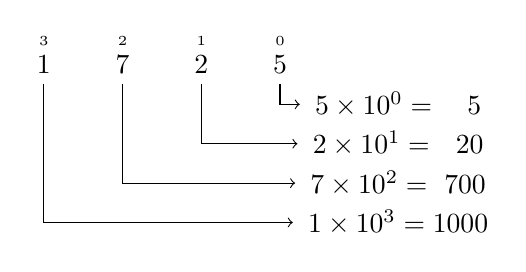
\begin{tikzpicture}[
  flow/.style={draw=black,->,shorten >=2pt}
]
  \node (s3) at (0, 2.3) {\tiny 3};
  \node (s2) at (1, 2.3) {\tiny 2};
  \node (s1) at (2, 2.3) {\tiny 1};
  \node (s0) at (3, 2.3) {\tiny 0};

  \node (n3) at (0, 2) {1};
  \node (n2) at (1, 2) {7};
  \node (n1) at (2, 2) {2};
  \node (n0) at (3, 2) {5};

  \node (e3) at (4.5, 0.0) {$1 \times 10^3 = 1000$};
  \node (e2) at (4.5, 0.5) {$7 \times 10^2 = ~700$};
  \node (e1) at (4.5, 1.0) {$2 \times 10^1 = ~~20$};
  \node (e0) at (4.5, 1.5) {$5 \times 10^0 = ~~~5$};

  \draw[flow] (n3.south) |- (e3.west);
  \draw[flow] (n2.south) |- (e2.west);
  \draw[flow] (n1.south) |- (e1.west);
  \draw[flow] (n0.south) |- (e0.west);
\end{tikzpicture}
\end{center}
\end{tcolorbox}

Wir beginnen dabei, die einzelnen Ziffern unserer Zahl \emph{von rechts} zu nummerieren und beginnen dabei mit der null. Die \enquote{Wertigkeit} jeder einzelnen Ziffer ergibt sich aus dem Wert der Ziffer und ihrer Position: Sie ist jeweils das Produkt aus Ziffer und einer \emph{Zehnerpotenz}. Die gesamte Zahl ist dann die Summe der einzelnen Wertigkeiten.

Nach demselben Muster funktioniert die Interpretation einer \emph{Binärzahl}. Ziffern (\emph{Bits}) können allerdings nur die Werte 0 oder 1 annehmen. Die Wertigkeit ergibt sich aus der Multiplikation mit einer \emph{Zweierpotenz}. Betrachten wir zum Beispiel die Darstellung der Dezimalzahl $42 = 32 + 8 + 2$ als Binärzahl:
\begin{tcolorbox}
	[title=Interpretation der Dezimalzahl 42 als Binärzahl,
	 arc=0pt,
	 outer arc=0pt
	]
\begin{center}
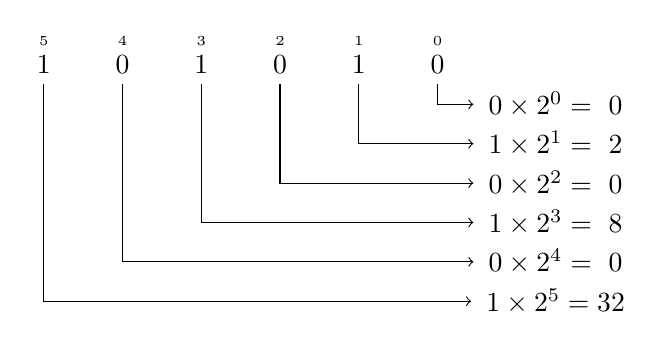
\begin{tikzpicture}[
  flow/.style={draw=black,->,shorten >=2pt}
]
  \node (s5) at (0, 3.3) {\tiny 5};
  \node (s4) at (1, 3.3) {\tiny 4};
  \node (s3) at (2, 3.3) {\tiny 3};
  \node (s2) at (3, 3.3) {\tiny 2};
  \node (s1) at (4, 3.3) {\tiny 1};
  \node (s0) at (5, 3.3) {\tiny 0};

  \node (n5) at (0, 3) {1};
  \node (n4) at (1, 3) {0};
  \node (n3) at (2, 3) {1};
  \node (n2) at (3, 3) {0};
  \node (n1) at (4, 3) {1};
  \node (n0) at (5, 3) {0};

  \node (e5) at (6.5, 0.0) {$1 \times 2^5 = 32$};
  \node (e4) at (6.5, 0.5) {$0 \times 2^4 = ~0$};
  \node (e3) at (6.5, 1.0) {$1 \times 2^3 = ~8$};
  \node (e2) at (6.5, 1.5) {$0 \times 2^2 = ~0$};
  \node (e1) at (6.5, 2.0) {$1 \times 2^1 = ~2$};
  \node (e0) at (6.5, 2.5) {$0 \times 2^0 = ~0$};

  \draw[flow] (n5.south) |- (e5.west);
  \draw[flow] (n4.south) |- (e4.west);
  \draw[flow] (n3.south) |- (e3.west);
  \draw[flow] (n2.south) |- (e2.west);
  \draw[flow] (n1.south) |- (e1.west);
  \draw[flow] (n0.south) |- (e0.west);
\end{tikzpicture}
\end{center}
\end{tcolorbox}

\begin{figure}[b!]
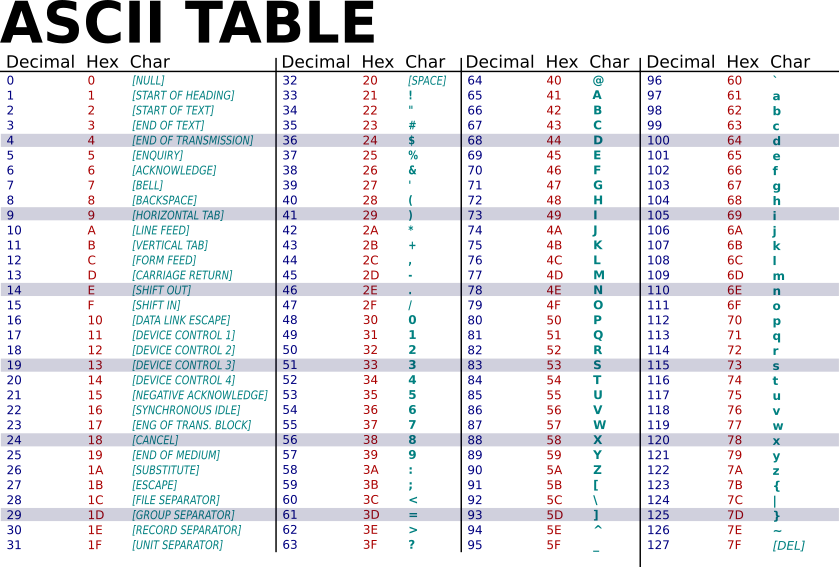
\includegraphics[width=\linewidth]{./gfx/ASCII_table}\newline
\caption
	[ASCII-Codes]
	{ASCII: American Standard Code for Information Interchange\newline
         Quelle: \url{https://commons.wikimedia.org/wiki/File:ASCII-Table-wide.svg}
    }
\label{fig:ASCII}
\end{figure}
Texte werden intern als Folge von Zahlen behandelt. Jedem Zeichen wird eine Zahl zugeordnet und mittels einer Tabelle \enquote{übersetzt}. Aus technischen Gründen ist die Zahl der darstellbaren Zeichen für einfache Programme auf 256 begrenzt\footnote{In der Vorlesung \emph{Algorithmen und Datenstrukturen} an der Universität Regensburg erfahren Sie, wie Sie diese Schranke umgehen und so \eg internationale Schriftzeichen in ihren Programmierprojekten verwerten. Sie können sich hierzu auch selbst Wissen zum Stichword \emph{Unicode} aneignen.}. Davon sind die ersten 128 Zuordnungen international genormt; die zweite Hälfte der Tabelle hängt von den Ländereinstellungen am jeweiligen Rechner ab. Siehe Abb.\,\ref{fig:ASCII} für die Zuordnung.

Damit können wir mit den Mitteln der Elektronik bereits (nahezu) beliebig große positive Ganzzahlen und Schriftzeichen darstellen\footnote{negative Zahlen und Dezimalbrüche werden in Abschnitt \ref{sec:Datawidth} behandelt}. Wie aber schafft man es, aus Zahlen komplexe Programme zu bauen?

\section{Von Zahlen zu Befehlen} \label{sec:assembly}
Die \emph{CPU} (Central Processing Unit) eines Computers ist ein elektronisches Bauteil, in dem eine gewisse Anzahl sehr einfacher Arbeitsschritte \enquote{mechanisch} im Chip umgesetzt sind. Solche Arbeitsschritte sind etwa \enquote{addiere zwei Zahlen} oder \enquote{lade einen Wert vom Speicher}. Diese Befehle kann man sich als \enquote{durchnummeriert} denken. Ist \texttt{17} beispielsweise die Nummer des Befehls \texttt{multipliziere}, so drückt die Zahlenkette \texttt{17 21 2} also den Auftrag \texttt{multipliziere die Zahlen 21 und 2 miteinander} aus. Genau aus solchen Zahlenketten besteht jedes Computerprogramm. Die Zahlen werden im \emph{Binärformat} gespeichert, also als Kette von 0en und 1en, die auch als Schriftzeichen interpretiert werden könnten. Öffnet man mit einem Textbearbeitungsprogramm eine ausführbare Datei, so zeigt dieses nur einen unverständlichen Zeichensalat an. Für einen Menschen wäre es beschwerlich, eine solche Datei zu lesen; theoretisch ist es aber möglich, mithilfe einer geeigneten Tabelle ausführbare Dateien zu \enquote{lesen}.

In den Pioniertagen der Computertechnik musste man tatsächlich die Zuordnung der Zahlen zu den Befehlen kennen, um ein Computerprogramm zu schreiben. Diese Arbeitsweise ist selbstverständlich sehr umständlich und fehleranfällig. Erste Abhilfe schuf hier die Programmiersprache \emph{Assembler}. Jedem CPU-Befehl wurde ein kurzer Text (ein sog. \emph{Mnemonic}) zugeordnet. Befehle wie \texttt{mul 21 2} erlauben bereits bedeutend komfortableres Schreiben und Warten von Programmen.

Die Programmierung in Assembler ist anspruchsvoll und erlaubt es kaum, komplexe Projekte umzusetzen\footnote{Die erste Generation der Gameboy-Spielereihe \emph{Pokémon} wurde in Assembler programmiert. Obgleich dies eine beachtliche Leistung darstellt sind diese Spiele heute bekannt für die Vielzahl von in diesen enthaltenen \emph{Glitches} (Fehlern im Code, die unbeabsichtigte Effekte auslösen).}. Aus diesem Grund wurden \emph{Hochsprachen} wie C entwickelt, in denen komplette \enquote{Arbeitspakete} wie \enquote{Gib einen Text auf dem Bildschirm aus} in einem einzelnen Befehl zusammengefasst sind. Damit diese C-Befehle vom Computer verstanden werden, müssen diese natürlich erst wieder in Maschinensprache zurückübersetzt werden, also in eine Folge von Zahlen, die die CPU interpretieren kann. Diese Aufgabe benutzt ein sogenannter \emph{Compiler}, also ein spezielles Computerprogramm\footnote{Tatsächlich wird häufig erst von der Hochsprache in Assembler übersetzt. Der letzte Schritt -- die Übersetzung von Assembler-Code in Maschinensprache -- übernimmt ein \emph{Assembler}. In der Praxis sagt man aber einfach \enquote{kompilieren} zur Gesamtheit aller Übersetzungsschritte bis hin zur Maschinensprache.}.

Ein Vorteil von Hochsprachen ist, dass man eigene Funktionen für komplexe Aufgaben realisieren kann. Häufig wiederkehrende Aufgaben werden in sogenannten \emph{Bibliotheken} oder \emph{Libraries} gesammelt und -- oft schon \emph{vorkompiliert} (also bereits in Maschinensprache übersetzt) -- anderen Programmierern zur Verfügung gestellt. So existiert in C beispielsweise die  \emph{math-library}, in der Operationen wie \emph{finde die Quadratwurzel einer Zahl} umgesetzt werden. Ein sogenannter \emph{Linker} sorgt dafür, dass Code aus eigenen Projekten und vordefinierten Libraries korrekt verknüpft werden.

\section{Aufruf des Compilers} \label{sec:Compile}
Für diesen Kurs benutzen wir den \emph{GNU C-Compiler} (gcc). Dieses Programm ist sowohl ein Compiler als auch ein Linker. Gehen wir davon aus, im aktuellen Arbeitsverzeichnis liegt eine Datei mit dem Namen \texttt{myCode.c} vor. Diese Datei kann kompiliert werden mit dem Kommandozeilen-Befehl:
\begin{cmdbox}[Kommandozeilen-Befehl: Kompilieren]
gcc myCode.c
\end{cmdbox}

Der gcc kompiliert mit diesem Befehl die Datei \texttt{myCode.c} und erstellt eine ausführbare Datei mit dem Dateinamen \texttt{a.out}. Diese kann nun über den Kommandozeilen-Befehl:
\begin{cmdbox}[Kommandozeilen-Befehl: Kompiliertes Programm ausführen]
./a.out
\end{cmdbox}
ausgeführt werden. Besteht der Code aus mehreren \emph{Modulen}\footnote{\ie mehrere Dateien; im Detail steckt mehr hinter diesem Begriff, worauf wir in Kapitel \ref{chp:modules} näher eingehen werden.}, so können diese einfach beim Aufruf des gcc hintereinander durch Leerzeichen getrennt aufgelistet werden. Neben Quellcode-Dateien (Erweiterung \texttt{.c}) können auch vorkompilierte \enquote{Object Codes} (Erweiterung \texttt{.o}) aufgelistet werden.
\begin{cmdbox}[Kommandozeilen-Befehl: Kompilieren mehrerer Module]
gcc myCode.c otherCode.c moreCode.c objectFile.o otherObject.o
\end{cmdbox}

In jedem Beispiel wird eine Datei \texttt{a.out} erstellt (bzw. überschrieben, falls diese bereits existiert). Möchte man, dass das kompilierte Programm einen anderen Namen erhält, so kann die Option \texttt{-o [OutputName]} angegeben werden; \texttt{[OutputName]} ist dabei der neue Dateiname. Beispiel: die zu erstellende ausführbare Datei soll den Namen \texttt{myProgram} tragen:
\begin{cmdbox}[Kompilieren mit vorgegebenem Dateinamen für das kompilierte Programm]
gcc -o myProgram myCode.c
\end{cmdbox}
Man startet dieses Programm dann mit dem Kommando
\begin{cmdbox}[Kommandozeilen-Befehl: Kompiliertes Programm ausführen]
./myProgram
\end{cmdbox}

Während der Entwicklung eines Programmes wird man häufig Fehler machen. Manche dieser Fehler sorgen für Code, der vom Compiler nicht interpretiert werden kann; man spricht \ua von \emph{Syntaxfehlern}. Dies können beispielsweise fehlende Klammern sein. Enthält der Code solche Fehler, wird das Kompilieren abgebrochen und keine ausführbare Datei erzeugt. Stattdessen zeigt der Compiler Informationen zum Fehler in der Kommandozeile an. (Wir gehen in den folgenden Kapiteln genauer auf diese Rückmeldungen ein).

Andere Code-Elemente können zwar in \enquote{validen Maschinencode} umgesetzt werden, enthalten aber evtl. logische Fehler (sog. \emph{semantische Fehler}). Standardmäßig gibt der Compiler hierzu keine Rückmeldung. Wir können aber mit den Kommandozeilenoptionen\footnote{Compiler Optionen werden oftmals auch \emph{Compiler Flags} genannt.} \texttt{-Wall}, \texttt{-Wimplicit-fallthrough} und \texttt{-Wpedantic} einstellen, dass auf solche Strukturen in der Compiler-Ausgabe ebenfalls hingewiesen werden soll. In der Compiler-Ausgabe werden diese dann als \emph{warnings} vermerkt (daher das \texttt{W} in \texttt{Wall}, \texttt{-Wimplicit-fallthrough} und \texttt{Wpedantic}). Ich empfehle sehr, diese Optionen zu nutzen und den Code zu verbessern, bis alle Warnungen beseitigt sind; in meinen Projekten haben diese Optionen einige Fehler aufgedeckt und mir viel Zeit erspart.

Ein Aufruf mit diesen Optionen sieht also so aus:
\begin{cmdbox}[Kompilieren mit Ausgabe aller Warnungen]
gcc -Wall -Wimplicit-fallthrough -Wpedantic -o myProgram myCode.c
\end{cmdbox}

Bibliotheken (\eg \texttt{.o}-Dateien) liegen in der Regel nicht im aktuellen Arbeitsverzeichnis, sondern in einem Standard-Verzeichnis, so dass alle Codes auf der Festplatte diese gleichermaßen Nutzen können. Um dem Compiler mitzuteilen, dass eine solche Bibliothek mit in den Linking-Prozess einbezogen werden soll, benutzen wir die Kommandozeilen-Option \texttt{-l[library]}, wobei \texttt{[library]} der Name der Bibliothek ist, die einbezogen werden soll. Im Kurs wollen wir \eg desöfteren mathematische Funktionen aus der Mathe-Bibliothek \texttt{libm} benutzen. Entsprechend ergänzen wir den Compiler-Aufruf um die Option \texttt{-lm}. Das voranstehende \texttt{lib} wird vom Compiler automatisch entfernt:
\begin{cmdbox}[Kompilieren und Linken mit der math-library]
gcc -Wall -Wimplicit-fallthrough -Wpedantic -o myProgram -lm myCode.c
\end{cmdbox}

Im Vorwort wurde erwähnt, dass C laufend fortentwickelt wird. Dies hat Auswirkungen auf die Interpretation des Codes; derselbe Code wird von älteren Versionen des Compilers nicht zwangsweise in derselben Art umgesetzt wie von neueren. Der gcc kann sowohl nach älteren als auch neueren Versionen der Sprache C kompilieren. Welche Version der Sprache benutzt werden soll, wird mit der Kommandozeilenoption \texttt{-std=[standard]} angegeben. Im Kurs halten wir uns an den Standard aus dem Jahr 2011, und ergänzen den Kommandozeilen-Aufruf entsprechend um \texttt{-std=c11}:
\begin{cmdbox}[Kompilieren mit nach Standard C11]
gcc -std=c11 -Wall -Wimplicit-fallthrough -Wpedantic -o myProgram myCode.c -lm
\end{cmdbox}

Neben den gezeigten Optionen existieren noch viele weitere Schalter, über die die Arbeitsweise des Compilers beeinflusst werden können; auf diese soll hier jedoch nicht weiter eingegangen werden. Interessierte KursteilnehmerInnen können mit dem Befehl \texttt{man} eine Übersicht aller Optionen mit Erklärungen anzeigen lassen.
\begin{cmdbox}[man-page des gcc]
man gcc
\end{cmdbox}

\begin{plusbox}
Die hier gegebenen Erklärungen und Optionen gelten so auch für C++. Jedoch sollte der Compiler \texttt{g++} benutzt werden. Das heißt, an allen Stellen, in denen oben \texttt{gcc} stand, muss durch \texttt{g++} ersetzt werden. Außerdem muss als Standard  dann \texttt{-std=c++11} anstelle von \texttt{-std=c11} angegeben werden.
\end{plusbox}

\begin{hintbox}
Da es lästig werden kann, wiederholt dieselben Optionen zu tippen, arbeite ich für kleinere Projekte gerne mit einem kleinen Script wie dem folgenden\footnote{Für größere Projekte gibt es Mechaniken, die hier nicht angesprochen werden können. Interessierte KursteilnehmerInnen können die DozentInnen bei Interesse auf \emph{makefiles} ansprechen.}:
\begin{codebox}[Mini-Script \texttt{compile} zum komfortablen kompilieren]
\begin{minted}[linenos]{bash}
OPTIONS="-std=c11 -Wall -Wimplicit-fallthrough -Wpedantic"
LIBS="-lm -lncurses"

INFILE=$1
OUTFILE="${INFILE%%.*}"

clear

rm -f $OUTFILE
echo ==================================
echo attempting to compile
echo gcc $OPTIONS -o $OUTFILE $INFILE $LIBS
echo ..................................
echo ""

gcc $OPTIONS -o $OUTFILE $INFILE $LIBS

echo ""
echo ..................................
echo Compilation successfull.
echo ..................................
echo ""
./$OUTFILE
\end{minted}
\end{codebox}

Dieses Script kann \eg in einer Textdatei mit Namen \texttt{compile} gespeichert und als ausführbares Script markiert werden. Letzeres geschieht über einen Kommandozeilen-Befehl:
\begin{cmdbox}[Kommandozeile: Script ausführbar machen]
chmod +x ./compile
\end{cmdbox}

Mit diesen Schritten reicht es, nur noch
\begin{cmdbox}[Kommandozeile: Script ausführen]
./compile myCode.c
\end{cmdbox}
einzugeben. Der Code automatisch mit den besprochenen Optionen kompiliert und direkt ausgeführt, sofern der Code erfolgreich kompiliert werden konnte.
\end{hintbox}
